\chapter{Ordering in Inherent Structures}

In the previous chapter we investigated the dynamics of three molecular systems. The dynamic properties of these systems remained smooth throughout the range we simulated them, there were no discontinuities indicating that there was no phase transition taking place. While there is no obvious phase transition, one possible cause of the increasing time scale for the dynamic properties is the growth of ordered regions within the simulations.

The goal of this chapter is to investigate the structural properties of the three systems studied in the previous chapter to determine whether the dynamic properties observed are purely dynamic properties or can be attributed to structural properties of the system.

\section{Do the Structures Remain Amorphous?}

Over the course of the simulations to determine the dynamic properties of the system it is possible that the system transitioned from the purely amorphous phase to a structure that was a mixture of crystalline and amorphous regions. If these regions are long lived, rather than just fluctuations, as the temperature is dropped these regions are only more likely to grow; the lower entropy crystal phase is more favourable at low temperatures. Using this reasoning we can use the final configuration as an indication of the formation of crystalline regions over the entire temperature range of the simulation. From this final configuration we can take an inherent structure, removing any of the vibrational noise giving a configuration that is representative of the mean arrangement of the molecules. These inherent structures for each molecule are shown in \textfigref{inherent structures frame} where the colour of each molecule denotes its orientation. The three molecules have different behaviours, the \sone molecule \figref{sone inherent} shows many regions of orientational order, where molecules are arranged in layers with the orientation of molecules alternating between layers forming a p2mg unit cell. The presence of crystallisation in the inherent structure of the \sone molecule indicates that our initial assessment of being a poor crystalliser was incorrect. The \scon molecule \figref{scon inherent} seems to show no long range ordering, there are small regions of about five molecules where there is antiparallel ordering, a p2 unit cell, however these regions are terminated with regions of random orientation. The size of the ordered regions is more indicative of a local structural phenomenon rather than long range crystal formation. The final molecule \tri \figref{tri inherent} shows no sign of crystallisation from a visual inspection. While visual inspection is a useful tool, providing us with a starting point for analysis and elucidating unexpected results, more specialised techniques need to be used to fully understand the structural properties of these inherent structures.

\begin{figure}
    \centering
    \begin{subfigure}{0.45\linewidth}
        \zoom{2}{Snowman-0.65-0.637556-1.0-frame-0320000181}
        \caption{The configuration of \sone shows regions of orientational order with layers of molecules arranged antiparallel to each other. These regions have different orientations indicating a series of nucleation events.}
        \label{fig:sone inherent}
    \end{subfigure}
    \begin{subfigure}{0.45\linewidth}%
        \zoom{2}{Snowman-1.55-0.637556-1.637556-frame-0320000182}
        \caption{The \scon molecule shows no sign of long range order. There are small clusters of about five particles exhibiting antiparallel ordering, although not large enough to be considered nucleation.}
        \label{fig:scon inherent}
    \end{subfigure}
    \begin{subfigure}{0.45\linewidth}
        \zoom{2}{Trimer-1.15-0.637556-1.00-120-frame-0320000198}
        \caption{The \tri molecule shows no sign of ordering, a truly amorphous phase.}
        \label{fig:tri inherent}
    \end{subfigure}
    \caption{Final inherent structure configurations for each molecule, the colouring of the molecules representative of their orientations.}
    \label{fig:inherent structures frame}
\end{figure}

\subsection{Order Parameters}

There are a plethora of ways order can be measured in a system depending of the type of order that is expected to be present. The radial distribution function $G(r)$ is one of the more general techniques. The radial distributions \figref{radial distributions} of these concave molecules are unusually intense first shell peaks, far in excess of what would be expected. The intensity of these peaks can be attributed to the interaction of the molecules at the concavity, there is an intense peak in the COM distribution\figref{scon radial2d} around the concavities. While there are these strong short range interactions they do not lead to long range order, with the radial distributions only showing peaks out to the second shell. Beyond the second shell the distribution is uniform, matching that of an amorphous phase.

\begin{figure}
    \centering
    \begin{subfigure}{0.45\linewidth}
        \includegraphics[width=\linewidth]{{{Snowman-0.65-0.637556-1.0-radial}}}
        \caption{}
        \label{fig:sone radial}
    \end{subfigure}
    \begin{subfigure}{0.45\linewidth}
        \includegraphics[width=\linewidth]{{{Snowman-1.55-0.637556-1.637556-radial}}}
        \caption{}
        \label{fig:scon radial}
    \end{subfigure}
    \begin{subfigure}{0.45\linewidth}
        \includegraphics[width=\linewidth]{{{Trimer-1.15-0.637556-1.00-120-radial}}}
        \caption{}
        \label{fig:tri radial}
    \end{subfigure}
    \caption{}
    \label{fig:radial distributions}
\end{figure}

\begin{figure}
    \zoom{2}{Snowman-1.55-0.637556-1.637556-radial2d_rel}
    \caption{The two dimensional radial distribution of the \scon molecule. The intense inner peaks show the distribution of the COM when the molecules interact via the concavity.}
    \label{fig:scon radial2d_abs}
\end{figure}

Another measure of order is to look at the orientational distribution of the molecules.
\towrite{orientational order}

\begin{figure}
    \centering
    \begin{subfigure}{0.45\linewidth}
        \includegraphics[width=\linewidth]{{{Snowman-0.65-0.637556-1.0-angular}}}
        \caption{}
        \label{fig:sone angular}
    \end{subfigure}
    \begin{subfigure}{0.45\linewidth}%
        \includegraphics[width=\linewidth]{{{Snowman-1.55-0.637556-1.637556-angular}}}
        \caption{}
        \label{fig:scon angular}
    \end{subfigure}
    \begin{subfigure}{0.45\linewidth}
        \includegraphics[width=\linewidth]{{{Trimer-1.15-0.637556-1.00-120-angular}}}
        \caption{}
        \label{fig:tri angular}
    \end{subfigure}
    \caption{}
    \label{fig:angular distributions}
\end{figure}

\subsection{Order in \scon}

Both of the previous attempts at describing order in the compact packing were using the properties of a molecule, its orientation and center of mass. In both the ordered and random allocation of bonds the molecule is just a construct sitting atop a lattice of ordered particles. The particles define the arrangement and so using the particles to detect order within a configuration is a far more appropriate approach. Using the particles to define a 2D radial distribution function gives \textfigref{ordered radial2d, random radial2d} which are almost identical to each other. The energy and ordering of the structures is determined by the arrangement of the individual particles, not the arrangement of bonds.
\tofix{these paragraphs}
Consider the compact binary packing with a size ration of 0.637556:1; this is equivalent to packing the \scon molecule without the allocation of bonds. The allocation of bonds can be performed randomly with no adjustment to the structure of the underlying particles~\secref{compact degeneracy}. Two examples of assigning bonds; an ordered p2 structure~\figref{ordered frame}, and a randomly oriented structure~\figref{random frame}. The orientational order of the p2 structure can easily be seen with diagonal banding of colours, corresponding to the two orientations present in the structure. The randomly assigned structure has molecules arranged with no orientational order, distributed between the eight possible molecular orientations. We can attempt to remove the noise of this orientational disorder by only plotting the centers of mass~\figref{ordered com, random com}, however this gives a very similar result, the ordered structure exhibits distinctly crystalline behaviour with centers of mass aligning in rows while the random structure that needs further analysis to be considered ordered.

\begin{figure}
    \begin{subfigure}{0.5\linewidth}
        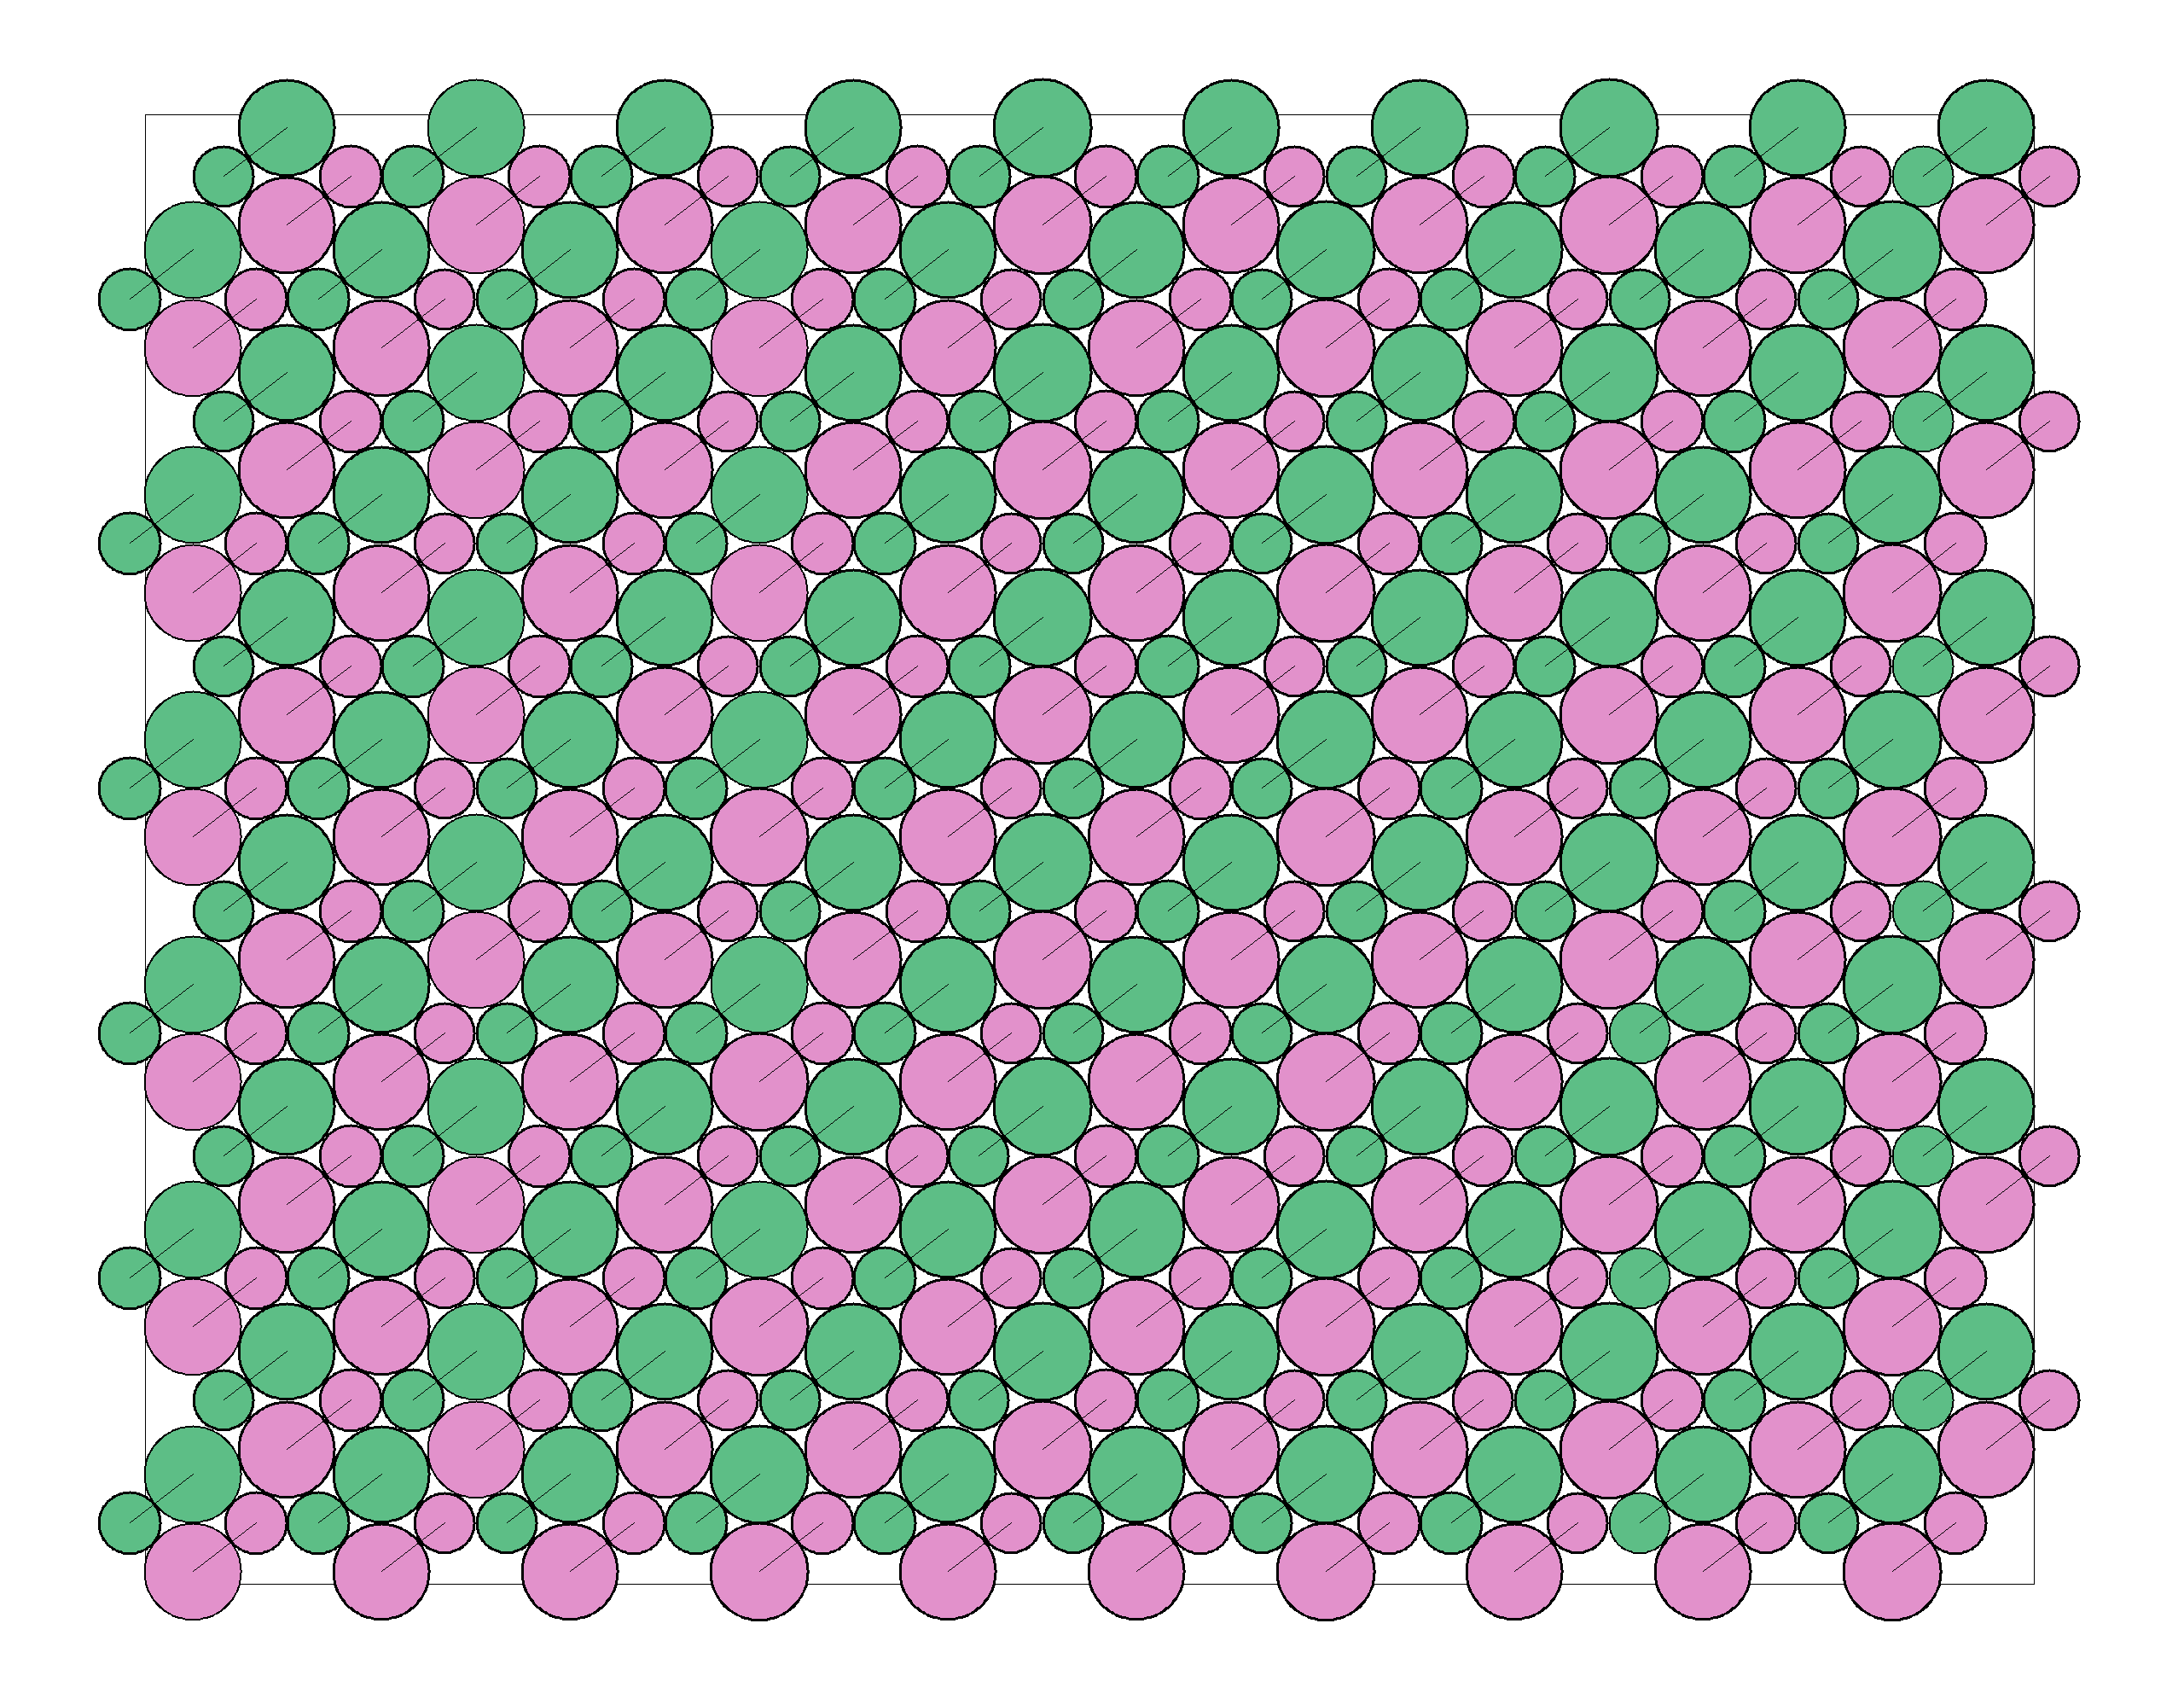
\includegraphics[width=\linewidth]{ordered-frame}
        \caption{Ordered frame}
        \label{fig:ordered frame}
    \end{subfigure}
    \begin{subfigure}{0.5\linewidth}
        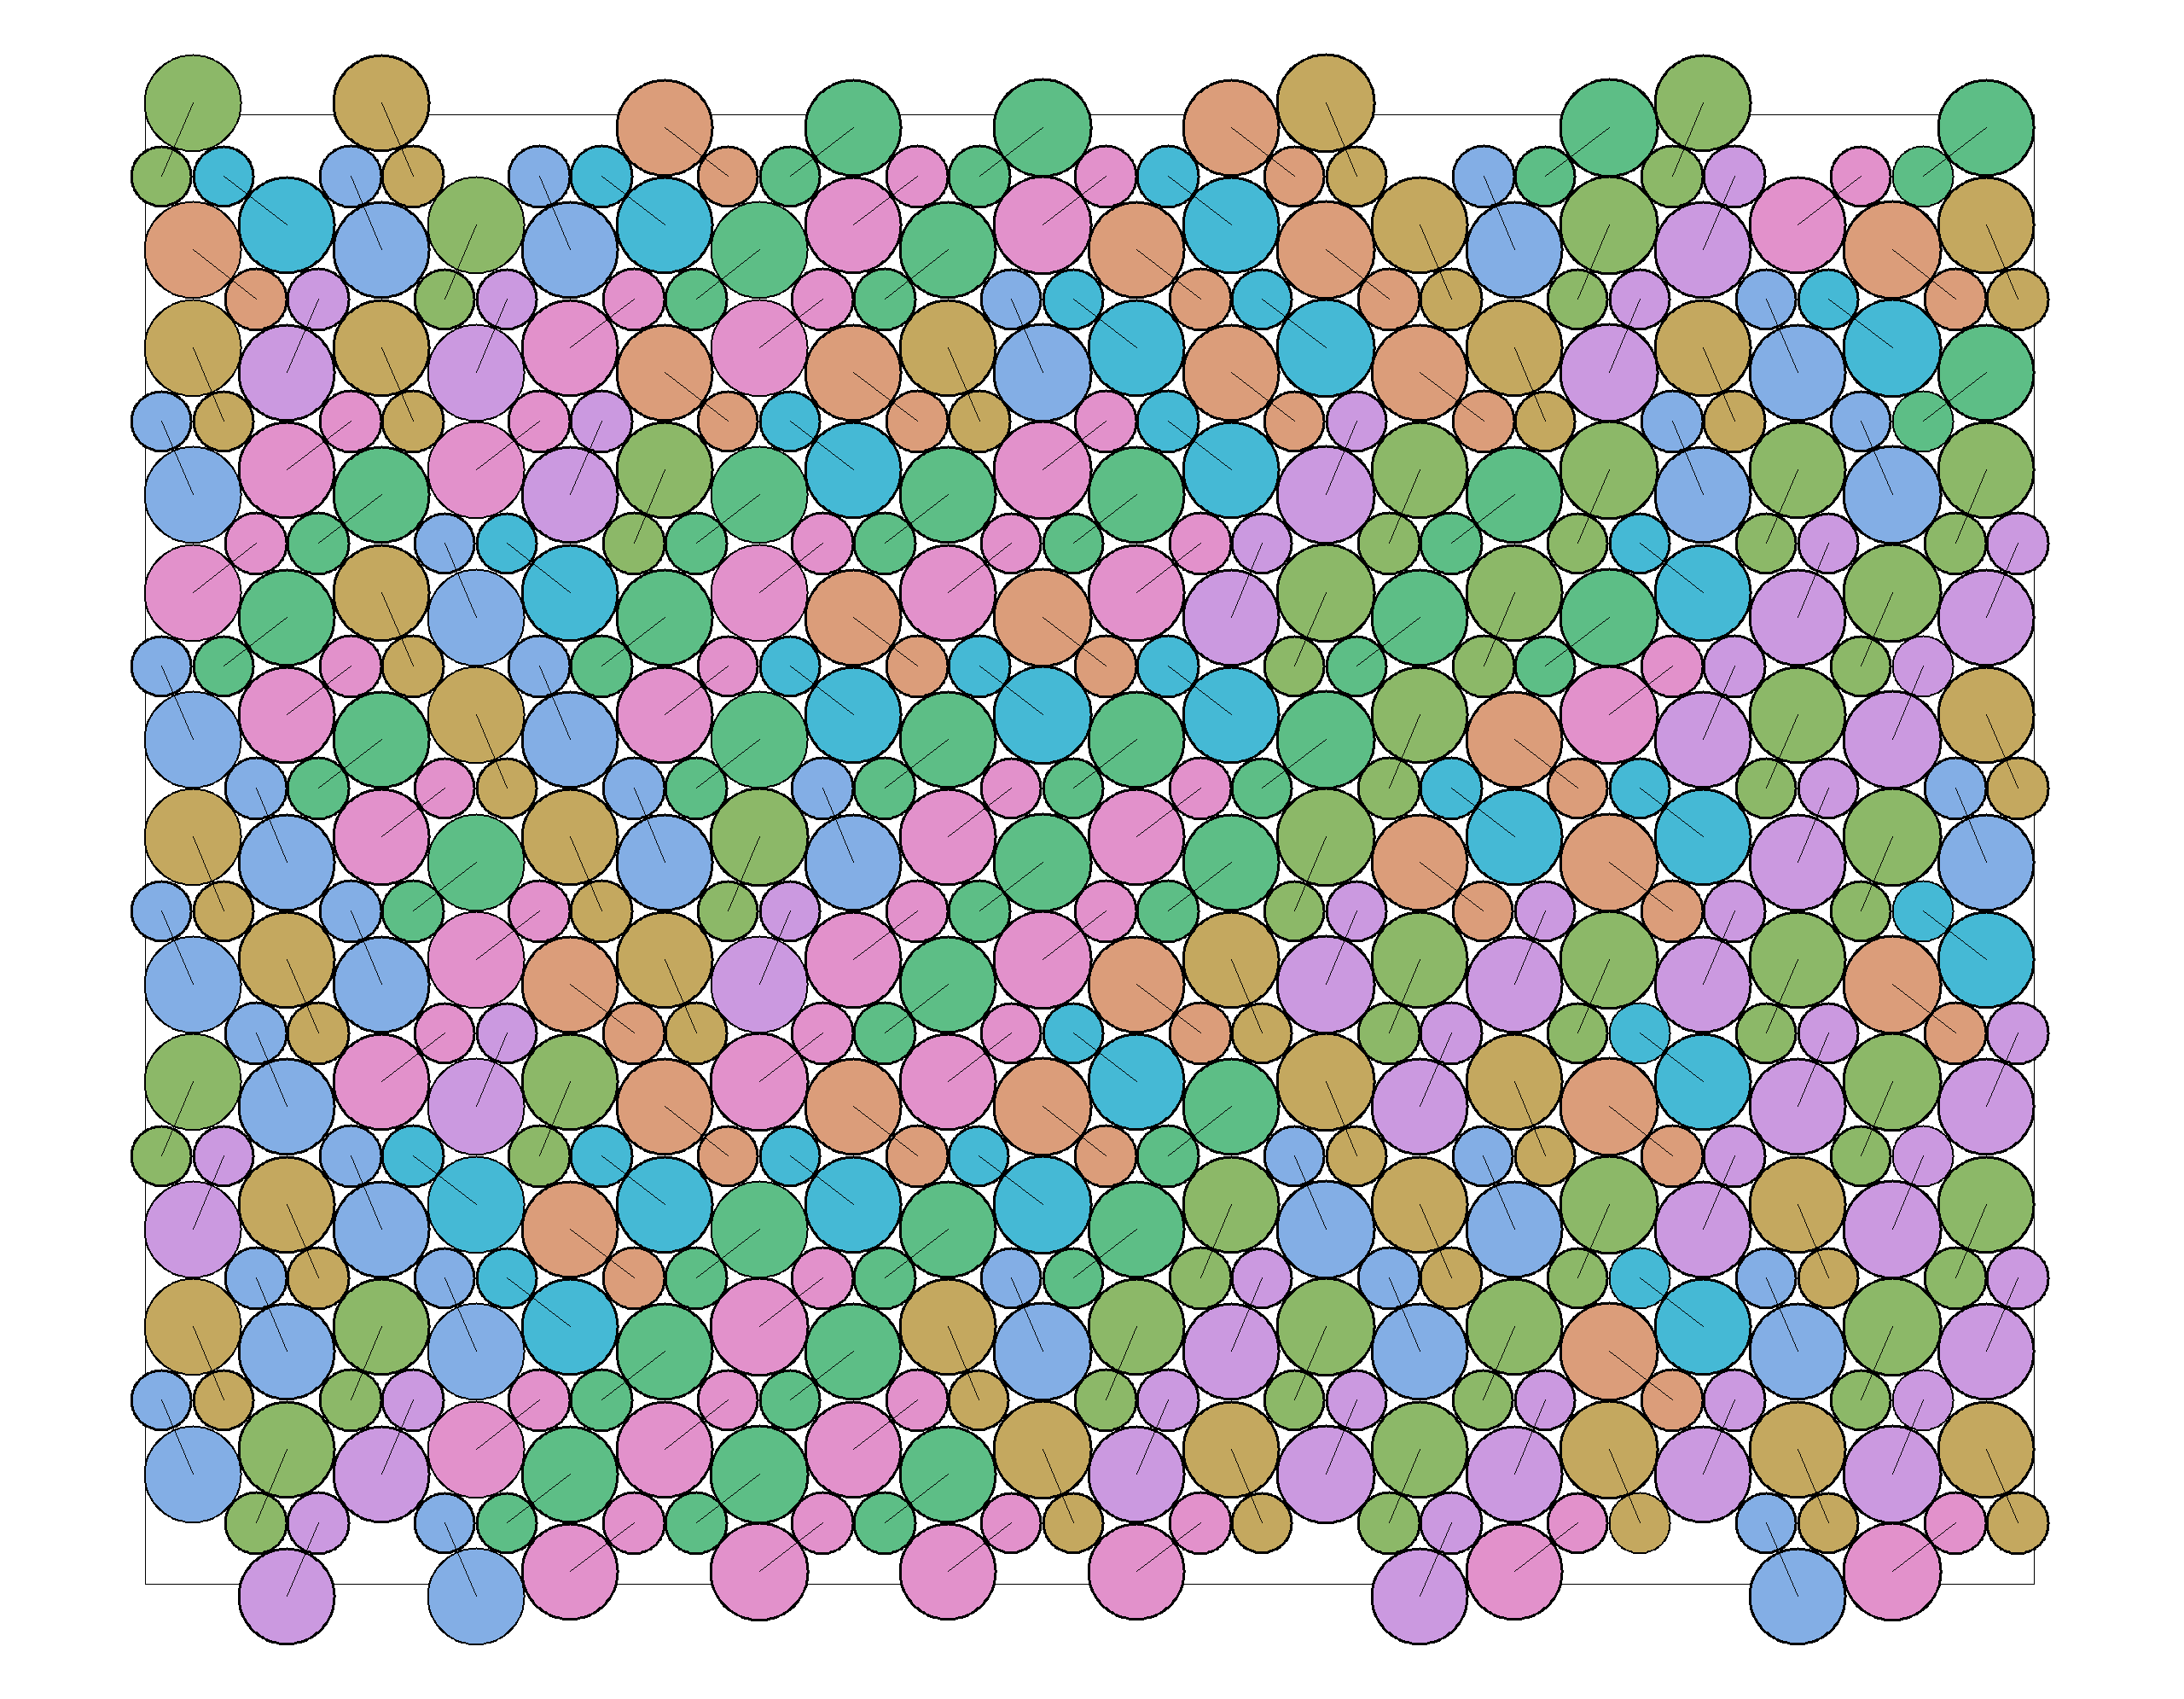
\includegraphics[width=\linewidth]{random-frame}
        \caption{Random frame}
        \label{fig:random frame}
    \end{subfigure}
    \begin{subfigure}{0.5\linewidth}
        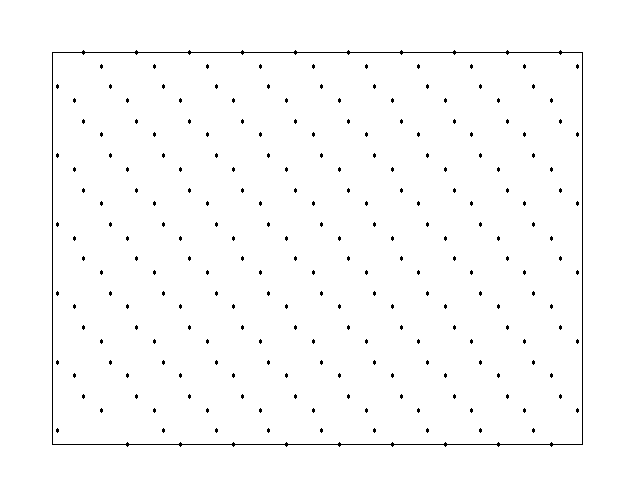
\includegraphics[width=\linewidth]{ordered-com}
        \caption{Ordered com}
        \label{fig:ordered com}
    \end{subfigure}
    \begin{subfigure}{0.5\linewidth}
        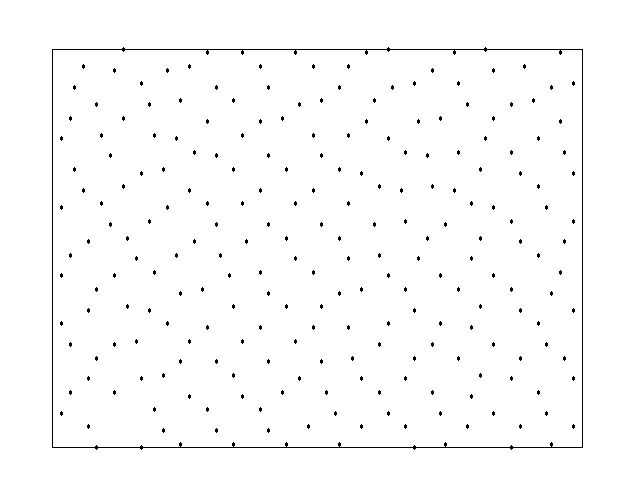
\includegraphics[width=\linewidth]{random-com}
        \caption{Random com}
        \label{fig:random com}
    \end{subfigure}
    \begin{subfigure}{0.5\linewidth}
        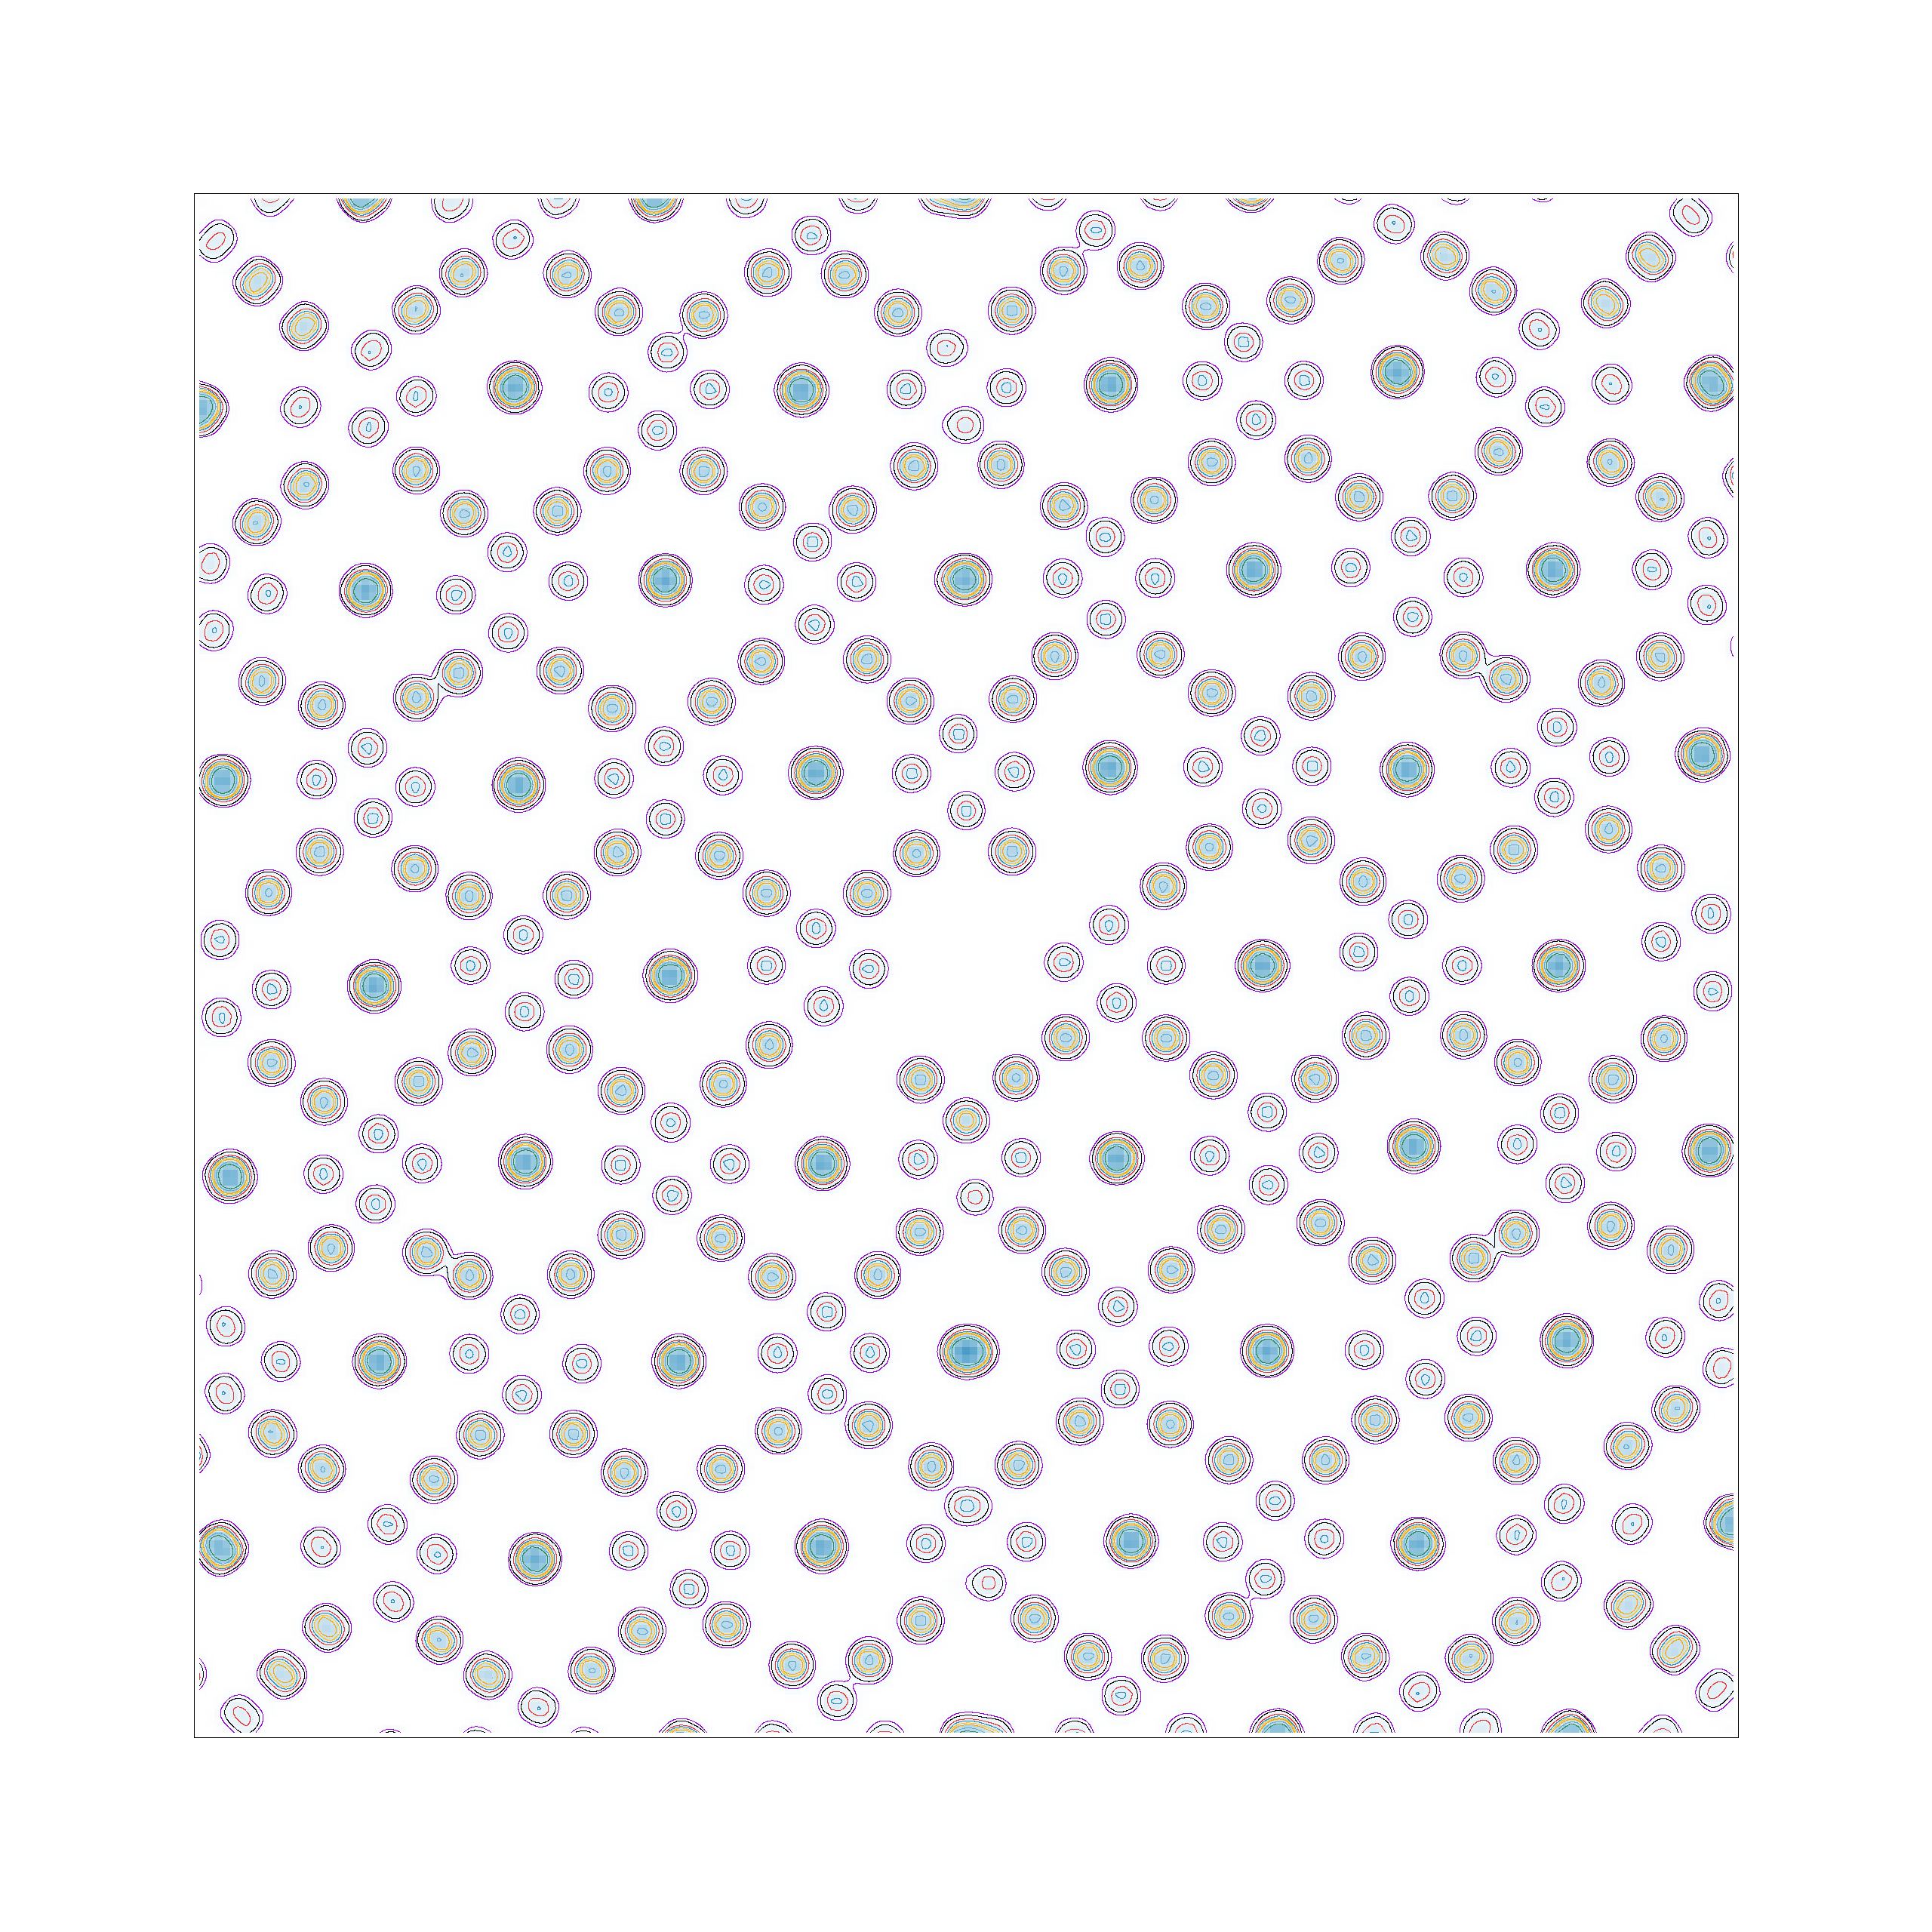
\includegraphics[width=\linewidth]{ordered-radial2d-part}
        \caption{Ordered radial2d}
        \label{fig:ordered radial2d}
    \end{subfigure}
    \begin{subfigure}{0.5\linewidth}
        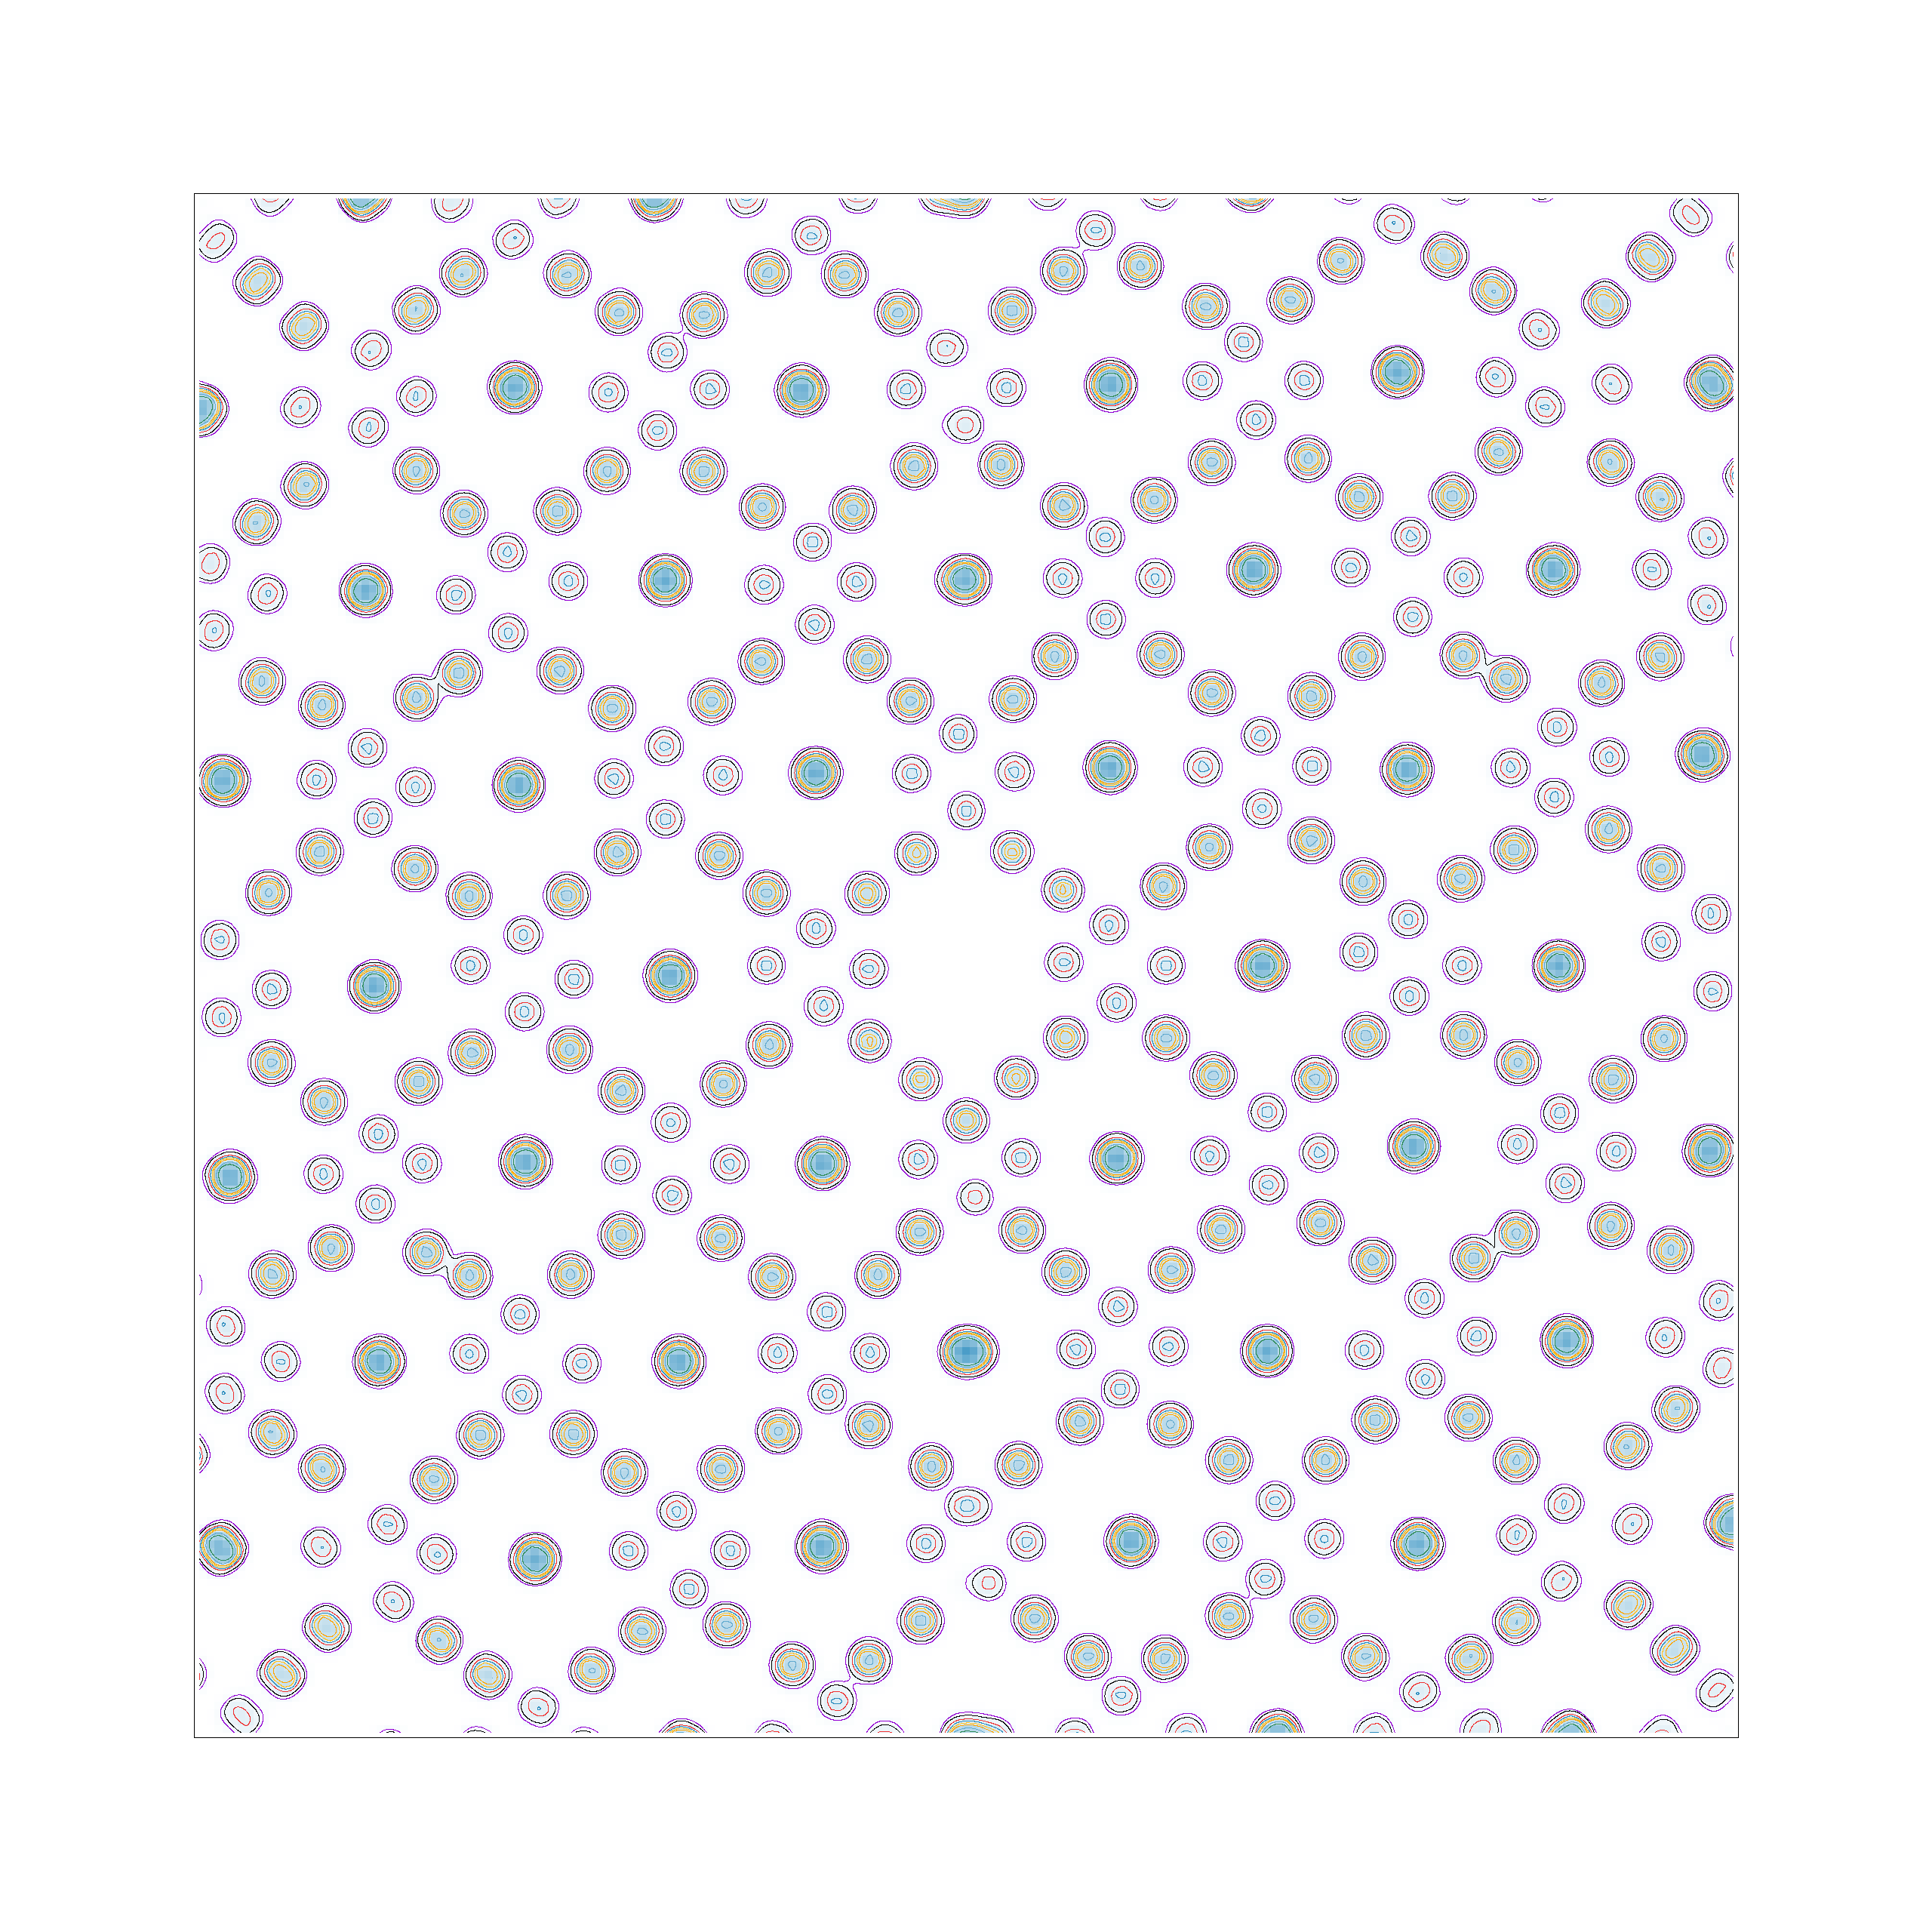
\includegraphics[width=\linewidth]{random-radial2d-part}
        \caption{Random radial2d}
        \label{fig:random radial2d}
    \end{subfigure}
    \caption{Comparison of crystalline and random assignment of bonds to a compact packing}
    \label{fig:compact bonds}
\end{figure}


Using this new order parameter
\towrite{interparticle ordering}

\begin{figure}
    \centering
    \begin{subfigure}{0.45\linewidth}
        \includegraphics[width=\linewidth]{{{Snowman-0.65-0.637556-1.0-radial_part}}}
        \caption{}
        \label{fig:sone radial2d}
    \end{subfigure}
    \begin{subfigure}{0.45\linewidth}
        \includegraphics[width=\linewidth]{{{Snowman-1.55-0.637556-1.637556-radial_part}}}
        \caption{}
        \label{fig:scon radial2d}
    \end{subfigure}
    \begin{subfigure}{0.45\linewidth}
        \includegraphics[width=\linewidth]{{{Trimer-1.15-0.637556-1.00-120-radial_part}}}
        \caption{}
        \label{fig:tri radial2d}
    \end{subfigure}
    \caption{}
    \label{fig:radial2d distributions}
\end{figure}

\section{What are the Lowest Energy Crystal Phases}

In the interests of developing more specialised tools for detecting crystalline order, we need to know which crystal structures are likely to form. This involves finding the lowest energy crystal structures. To find these lowest energy structures we need tools other than molecular dynamics since the timescales for molecular dynamics are beyond the limits of our simulations. To find a good approximation of the lowest energy structures we look to packing hard shapes, by modelling our molecules as hard shapes we are able to use an isopointal algorithm to get a good approximation of the closest packed configurations. These closest packed configurations can be used as the starting configuration for a Lennard-Jones system which is equilibrated at a low temperature to allow the crystals to relax before an inherent structure is taken to find the energies. \texttabref{crystal energies} shows the energy of the Lennard Jones systems using the best packed isopointal structures for each wallpaper group as a starting configuration. The Lennard-Jones system does not retain the constraints of the wallpaper group symmetry, however there are no significant deviations for the systems tabulated.

\begin{table}
    \sisetup{
        table-format = +3.4,
        table-omit-exponent,
        fixed-exponent =-4,
        parse-numbers=true,
        scientific-notation=true,
        round-mode=places,
        round-precision=3}
    \centering
    \begin{tabular}{ | l | S  S  S | }
        \hline
        {Crystal} & \multicolumn{3}{c|}{Energy per molecule (\num{e-4})} \\
            &\sone & \scon & \tri \\ \hline
        p2 & 0.00001376280055& \cellcolor{blue!20}0.0001527208398& \cellcolor{blue!10}-0.0003934685913\\
        p2mg & \cellcolor{blue!20}0.000005732595806& 0.0004479052484& -0.0003354198174\\
        p2gg & 0.00002632511042& 0.0001699363766& \cellcolor{blue!20}-0.000401823091\\
        pg & 0.00002824743917& 0.0002860863393& \cellcolor{blue!10}-0.0004000561542\\
        p3 & 0.00003468842645& 0.0002424453316& -0.0003292839541\\
        \hline
    \end{tabular}
    \caption{The energy per molecule for a variety of the best packing crystal structures. Both the \sone and \scon systems have an arrangement with significantly lower energy, p2mg and p2 respectively. While the \tri system has three arrangements with very similar energies, the p2, p2gg and pg wallpaper groups.}
    \label{tab:crystal energies}
\end{table}

From the energies in \texttabref{crystal energies} the most stable crystal structures are: \sone{} - p2mg, \scon{} - p2, and \tri{} - p2gg, with their repsectice configurations shown in \textfigref{crystals}. Interestingly these lowest energy structures are not necessarily the closest packed structures, it is possible the extra.
\towrite{energies}

\begin{figure}
    \centering
    \begin{subfigure}[t]{0.45\linewidth}
        \zoom{2}{Snowman-0.4-0.637556-1.00-p2mg-frame}
        \caption{}
        \label{fig:crystal sone}
    \end{subfigure}
    \begin{subfigure}[t]{0.45\linewidth}%
        \zoom{2}{Snowman-0.4-0.637556-1.637556-p2-frame}
        \caption{}
        \label{fig:crystal scon}
    \end{subfigure}
    \begin{subfigure}{0.45\linewidth}
        \zoom{2}{Trimer-0.4-0.637556-1.00-120-p2gg-frame}
        \caption{}
        \label{fig:crystal tri}
    \end{subfigure}
    \caption{}
    \label{fig:crystals}
\end{figure}


